\section*{\centering Reproducibility Summary}

% \textit{Template and style guide to \href{https://paperswithcode.com/rc2020}{ML Reproducibility Challenge 2020}. The following section of Reproducibility Summary is \textbf{mandatory}. This summary \textbf{must fit} in the first page, no exception will be allowed. When submitting your report in OpenReview, copy the entire summary and paste it in the abstract input field, where the sections must be separated with a blank line.
% }

\subsection*{Scope of Reproducibility}
% State the main claim(s) of the original paper you are trying to reproduce (typically the main claim(s) of the paper).
% This is meant to place the work in context, and to tell a reader the objective of the reproduction.
This report covers our reproduction of the paper 'Explaining Low dimensional Representation' \cite{plumb2020explaining} by Plumb et al. In this paper, a method (Transitive Global Translations, TGT) is proposed for explaining different clusters in low dimensional representations of high dimensional data. They show their method outperforms the Difference Between the Means (DBM) method, is consistent in explaining differences with few features and matches real patterns in data. We verify these claims by reproducing their experiments and testing their method on new data. We also investigate the use of more complex transformations to explain differences between clusters.



\subsection*{Methodology}
We reproduce the original experiments using their source code. We also replicate their findings by re-implementing the authors' method in PyTorch \cite{paszke2019pytorch} and evaluating on two of the dataset used in the paper and two new ones. Furthermore, we compare TGT with our own extension of TGT, which uses a larger class of transformations.

\subsection*{Results}
We were able to reproduce their results using their code, yielding mostly similar results. TGT generally outperforms DBM, especially when explanations use few features. TGT is consistent in terms of the features to which it attributes cluster differences, across different sparsity levels. TGT matches real patterns in data. When extending the types of functions used for explanations, performance did not improve significantly, suggesting translations make for adequate explanations. However, the scaling extension shows promising performance on the modified synthetic data to recover the original signal.


\subsection*{What was easy}
The easiest part was running the existing code with the pre-trained model files. The original authors had set up their code base in an organized manner with clear instructions.

\subsection*{What was difficult}

The first difficulty that we encounter was finding the right environment. The source code depends on deprecated functionality. The clustering method they used, had to be re-implemented for us to use it in our replication. Another difficulty was the selection of clusters. The authors did not prove a consistent method for selecting clusters in a latent space representation. When retraining the provided models, we get a latent space representation different to the original experiments. The clusters have to be manually selected. The metrics that they used to evaluate their explanations are also depend on the clustering. This means that there is some variability in the exact verification of reproducibility.

\subsection*{Communication with original authors}
We asked the original authors for clarification on how to choose the $\epsilon$ hyper-parameter. However, it became apparent that we had misread, and the procedure is indeed adequately reported in the paper.

\newpage

\section{Introduction}
% A few sentences placing the work in high-level context. Limit it to a few paragraphs at most; your report is on reproducing a piece of work, you don’t have to motivate that work.
The \textit{curse of dimensionality} \cite{bishop:2006:PRML} is a long-standing problem in Machine Learning. Data in many domains and applications (e.g. Bioinformatics) has high-dimensional representations. Finding patterns in such high-dimensional data is a challenging task. To this end, \textit{dimensionality reduction} \cite{xie2018survey} techniques have greatly helped in data-analysis, information extraction, building computational models, and in doing inference. Given an input $x \in \mathbb{R}^{d}$, dimensionality reduction learns a function $r: x \mapsto r(x), \;\; r(x)\in \mathbb{R}^{m}$, where $m<<d$. Such a dimensionality reduction function $r$ naturally arises in deep learning due to the expressivity and representational power of neural networks. The goal of $r$ is to encode useful knowledge about the input space, thus providing distinctive information in the transformed output $r(x)$. This results in ``clusters" or ``groups of points" in the transformation space. The downside of this exercise, however, is that the output space is usually non-interpretable. There is usually no easy way to know what information is present in the transformed points $r(x)$ and what sort of distinctive knowledge they contain. 

In this work, we reproduce the paper `Explaining Groups of Points in Low-Dimensional Representations' by Plumb et al. \cite{plumb2020explaining}. This paper proposes a method for explaining different clusters in latent space representation. They look at the problem of explaining the points in the latent space representation through the lens of Interpretability in Machine Learning. 
We reproduce their findings and expand upon their work with our an extension. We extend their research by applying their method to a larger class of explanation functions and testing their method on new dataset. We further investigate the efficacy of the explanations using a probing classifier \cite{belinkov-etal-2020-interpretability}.

\section{Methodology}
\label{sec:claims}
Counterfactual Explanations \cite{verma2020counterfactual} have emerged as an active research area in the field of Interpretable Machine Learning. A counterfactual explanation is defined as the smallest perturbation to the input that would change the output of a machine learning model. As such, these explanations are promising as they can provide suggestive recourse to the beneficiary in a machine learning based decision system.  As an interpretable machine learning problem, Plumb et al. \cite{plumb2020explaining} aim to find such counterfactual explanations in order to explain the differences between the groups in latent space. To this end, they employ the function $r$ itself to find what perturbation $\delta$ needs to be made to the input $x \in \real^{d}$ so that $r(x + \delta)$ belongs to the different target group. The goal is to find the \textit{global} explanations that apply to the whole group as opposed to the \textit{local} explanations which explain only individual examples \cite{carvalho2019machine}. 
% The problem addressed by Plumb et al. \cite{plumb2020explaining} is that clustering models, such as Variational Auto-Encoders (VAE's), can be very complex. It is difficult to interpret the parameters of linear layers with non-linear activation functions. 
% The authors contend that interpretability can only be satisfied by obtaining \textit{explanations} that are \textit{counterfactual}, by showing what specific features are the cause of two clusters being separated. 
Furthermore, the  explanations need to be \textit{sparse} for them to be interpretable by practitioners.
% Furthermore, they need to be global, by being valid for all members of the two clusters. 
Finally, these explanations should be be both \textit{symmetric} and \textit{transitive}. To obtain these \textit{Global Counterfactual Explanations}(GCE), the authors propose the algorithm called, Transitive Global Translations (TGT), explained hereafter.

Following the previous notation, let $r : \real^d \rightarrow \real^m$ denote our dimensionality reduction function, where $d$ is the dimensionality of the input space and $m$ is the latent space's dimensionality. Suppose $X_i, X_j \subset \real^d$ get mapped to the clusters $R_i, R_j \subset \real^m$ respectively. The goal is to define the transformation $t_{i \rightarrow j}: \real^{d} \to \real^{d}$ on $x \in X_{i}$ as $x^{'} = t_{i \to j}(x)$, so that $r(x^{'}) \in R_{j}$, or equivalently $x^{'} \in X_{j}$. 

% we would like to know how changes in the input features cause an input to be mapped to a certain cluster. We thus look for a function $t_{i \to j}: \real^d \to \real^d$ such that for $x_i \in X_i$ we have
% \[r(t_{i \to j}(x_i)) \in R_j\]

The proposed algorithm TGT considers the transformations of the form $t_{i \to j}(x) = x + \delta_{i \to j}$. To find the optimal parameters of the transformation function, authors imply a compressed-sensing based objective function as below:
\begin{equation} \label{loss_function}
   l(\delta_{i \to j}) = \norm{r(t_{i \to j}(\bar{X_i})) - \bar{R_j}}_2^2 + \lambda \norm{\delta_{i \to j}}_1
\end{equation}

where $\lambda \norm{\delta_{i \to j}}_1$ is a regularization term to incentivize sparser explanations, and $\bar{X_i} \in \real^{d}$ and $\bar{R_j} \in \real^{m}$ denote the means of the clusters in the input space and latent space respectively. Given clusters $0, 1, \ldots, n$, we get a total of $\frac{1}{2}n(n+1)$ transformations.
To further increase sparsity, we can truncate $\delta_{i \to j}$ to only the $k$ features with the largest absolute value, for some $k$. An issue with this is that the translation using the  truncated $\delta_{i \to j}$ might no longer correctly transform inputs that get mapped to $R_i$ into inputs that get mapped to $R_j$.

Furthermore, the transformations $t_{i \to j}$ have to adhere to several mathematical properties. Namely, for any clusters $i, j, k$ these transformations should be : a) Symmetric, i.e. $t_{i \to j} = \inverse{t_{j \to i}}$
and b) Transitive, i.e. $t_{j \to k} \circ t_{i \to j} = t_{i \to k}$. From these properties it follows that $t_{i \to i}$ is the identity function $\mathcal{I}$ as
\begin{equation}
   t_{i \to i} = t_{i \to 0} \circ t_{0 \to i} = t_{i \to 0} \circ \inverse{t_{i \to 0}} = \mathcal{I}  
\end{equation}
We define this condition as \textit{self-similarity}. Furthermore, the group of translations is uniquely defined by $t_{0 \to 1}, \ldots, t_{0 \to n}$, because for any $i, j$:
\begin{equation}
t_{i \to j} = t_{0 \to j} \circ t_{i \to 0} = t_{0 \to j} \circ \inverse{t_{0 \to i}}
\end{equation}

Plumb et al. \cite{plumb2020explaining} compare their method against the naive baseline of Difference Between the Means (DBM). With DBM, each transformation is still a translation: $t_{i \to j}(x) = x + \delta_{i \to j}$. However, now $\delta_{i \to j} = (\bar{X_j} - \bar{X_i})$. We also use this as a baseline for comparison in this report. 

Since translations are a very narrow class of functions, we expanded upon the research by investigating other transformations that still satisfy the GCE requirements. We investigate the transformations of the form $t_{0 \to i}(x) = \mathrm{exp}(\gamma_{0 \to i}) \odot x + \delta_{0 \to i}$. These always have a well defined inverse, given by $\inverse{t_{0 \to i}}(x) = \mathrm{exp}(-\gamma_{0 \to i}) \odot (x - \delta_{0 \to i})$ and only have $\bigo{d}$ parameters. The inclusion of scaling could enhance performance, while the necessary components of GCE are maintained.


\subsection{Metrics to evaluate Global Counterfactual Explanations}
\label{sec:metrics}
To measure the efficacy of the transformation function $t_{i \to j}$, the authors propose two metrics, \textit{Coverage} and \text{Correctness}. 
\begin{enumerate} \item The \textbf{Coverage} $\left(cv(t_{i \to j})\right)$ is the fraction of points $a \in R_j$ for which there is a point $b \in X_i$ such that $\norm{r(t_{i \to j}(b)) - a}_2 < \epsilon$, i.e.
\begin{equation}
  cv(t_{i \to j}) = \frac{1}{|R_{j}|}\sum_{a \in R_{j}}\mathbb{I}\left[ \exists  b \in X_{i} | \norm{r(t_{i \to j}(b) - a}_{2} < \epsilon \right]
\end{equation}
 \item The \textbf{Correctness} $\left(cr(t_{i\to j})\right)$  is the fraction of points $b \in X_i$ for which there is some $a \in R_j$ such that
 $\norm{r(t_{i \to j}(b)) - a}_2 < \epsilon$, i.e.
 \begin{equation}
  cr(t_{i \to j}) = \frac{1}{|X_{i}|}\sum_{a \in R_{j}}\mathbb{I}\left[ \exists  a \in R_{j} | \norm{r(t_{i \to j}(b) - a}_{2} < \epsilon \right]
\end{equation}
\end{enumerate}
Note that both these metrics have the hyperparameter $\epsilon$ which is to be chosen carefully. When $i=j$ we do not count the point itself, there must be some other point within distance $\epsilon$. \footnote{We use this definition to set the value for epsilon, as explained in the \textit{Methodology} section of the original Paper.}

Furthermore, the \textbf{Similarity} metric measures the consistency of the explanations at different sparsity levels. Given two explanations $e_1, e_2$ where $e_1$ is more sparse than $e_2$, the similarity of $e_1$ and $e_2$ is defined as
\begin{equation}
 sim(e_1, e_2) = \frac{\sum_i \abs{e_1[i]} \indc (e_2[i] \neq 0)}{\norm{e_1}_1}
\end{equation}
This is equal to $1$ if $e_1$ uses a subset of the features that $e_2$ uses. By definition, DBM always has similarity $1$.

\section{Scope of Reproducibility}
We investigate the following claims from the original paper:
\begin{enumerate}
    \item In terms of the average correctness and coverage, TGT performs equally well or better than the DBM method. This remains true, especially for sparser explanations.
    \item TGT explanations have similarity close to $1$. It is consistent in which features it uses for explanations across different sparsities.
    \item TGT correctly identifies known causal structure in data.
    \item Furthermore, TGT explanations are consistent. When altering the dataset by adding a copy of a cluster with a specific feature altered, TGT recovers the modification with little change to the other explanations.
\end{enumerate}


\section{Methodology of Reproducibility}

We make use of the code made available by the original authors \footnote{https://github.com/GDPlumb/ELDR} for our pilot investigative study. We first verify that the provided models and explanations stay true to the claims made in the paper. We further retrain their models on the provided dataset. We also made our own PyTorch \cite{paszke2019pytorch} implementation to to further verify the claims, and to perform experiments with the proposed extension.

\subsection{Model description}
We identify that the scope of the original paper is to explain clusters in the low-dimensional representations. However, obtaining meaningful and discernible low-dimensional representations is an active area of research. The original authors employ a t-SNE \cite{van2008visualizing} objective based Variational Autoencoder (called, henceforth, as scVIS) \cite{scvis} as the $r$ function. They make use of library\footnote{ \url{https://github.com/shahcompbio/scvis}} by the original scVIS authors in their implementation. We also implement this model in Pytorch for our experiments. However, we deliberately decide not to match the model implementation exactly. This is done to study the model-agnosticism of the TGT algorithm. By design, TGT should be able to explain the clusters for any differentiable $r$ function. However, we maintain that $r$ should give discernible latent representations with preserved global structure in the data. In our implementation of the scVIS library, we therefore do not employ the hyperparameters and the training settings from the original library. 

\subsection{Dataset Description}

We reproduce the findings of the authors on four datasets that they used. We use two of these datasets as well as two new ones to test our PyTorch implementation.
\begin{enumerate}
    \item \textbf{Single cell RNA} \cite{bipolar}: This dataset has $13166$ features. We use the same number of clusters at the original authors, $18$ in this case. 
    \item \textbf{UCI Boston housing} This dataset has 506 entries with 13 features. We use $6$ clusters for both reproduction and replication.
    \item \textbf{UCI Heart disease} This dataset has 303 entries with 13 features and 1 binary label. We used $8$ clusters in the reproduction and $4$ in the replication. The data was normalized to be in the range [0, 1]. 
    \item \textbf{UCI Iris} This dataset has 150 entries with 4 features and 1 ternary label. Ran in the reproduction with $3$ clusters. N = 150
    \item \textbf{Breast Cancer Wisconsin (Diagnostic) \footnote{https://www.kaggle.com/uciml/breast-cancer-wisconsin-data}} This dataset has 569 entries with 30 features and 1 binary label. We use $3$ clusters in the replication.
    \item \textbf{Pima Indians Diabetes Database} \footnote{https://www.kaggle.com/uciml/pima-indians-diabetes-database} This dataset has 768 entries with 8 features and 1 binary label. We used $3$ clusters in the replication. The data was normalized to be in the range [0, 1].

Note that the number of clusters depend on the latent-space representation, and thus, are user dependent.
    
\end{enumerate}
\subsection{Hyperparameters}
% Describe how the hyperparameter values were set. If there was a hyperparameter search done, be sure to include the range of hyperparameters searched over, the method used to search (e.g. manual search, random search, Bayesian optimization, etc.), and the best hyperparameters found. Include the number of total experiments (e.g. hyperparameter trials). You can also include all results from that search (not just the best-found results).

\paragraph{Tensorflow \cite{abadi2016tensorflow} Experiments}
For the reproduction of the original experiments, we use the same hyperparameters as the original authors.

\paragraph{Pytorch}
For our implementation of the scVIS model, we use l2 regularization of $0.001$, learning rate $0.01$, and perplexity of $10$. Furthermore, the degree-of-freedom for the studentT distribution is set to 2.0. Perplexity and the degree-of-freedom is used same as the original scVIS implementation. We use validation set to monitor the training process of the scVIS model, and stop training when the ELBO(Evidence Lower BOund)\cite{kingma2014autoencoding} stops improving. For training the TGT explanations, we closely follow the settings from Plumb et al. \cite{plumb2020explaining}. We initialize the deltas$\deltas_{s}$ as zero vectors. We tune the regularization parameter $\lambda$ by grid search over a fixed range $[0.0, 5.0]$ incremented by 0.5. Defining the metrics for TGT requires careful setting of the $\epsilon$ hyper-parameter.  We follow the \textit{self-similarity} condition (transformations of clusters to themselves should, theoretically, have correctness and coverage to be 1.0), and increase the $\epsilon$ in the range $[0.0, 2.0]$ with increments of 0.02 until the correctness and coverage metrics are greater than 0.95.  Furthermore, we use the truncation values(TV)(refer Table \ref{tab:tv}) to evaluate on the sparsity of the explanations. For the Pima Indians Diabetes Database and Breast Cancer Wisconsin(Diagnostic) dataset, we use the same truncation values as for UCI Boston Housing dataset.

\begin{table}[!ht]
    \centering
    \begin{tabular}{|c|c|c|}
    \hline
     \bf Dataset & \bf{Truncation Values(TV)} & \bf{$\epsilon$} \\
     \hline
        Single Cell RNA & 50, 100, 250, 500, 1000, 15000 & 0.75 \\
        \hline
        Heart Disease & 1, 3, 5, 7, 9, 11, 13 & 1.0 \\
        \hline
        Housing & 1, 3, 5, 7, 9, 11, 13 & 1.5 \\
        \hline
        Iris & 1, 2, 3, 4 & 0.75 \\
        \hline
    \end{tabular}
    \caption{Truncation Values (TV) and $\epsilon$ value used for each of the dataset.}
    \label{tab:tv}
\end{table}



\subsection{Experimental setup and code}
We closely follow the experimental setup in the original paper for our experiments. We make our Pytorch code available \footnote{https://github.com/elfrink1/FACT} to further support the reproducible research. We reran the code of the original authors with new clustering models and new explanations. We optimize the compressed-sensing based objective function for the TGT algorithm using the gradient descent algorithm. Our scaling extension is easily integrated in the source code, and can be optimized in a similar way. We train the scVIS models on the Lisa computing cluster \footnote{https://userinfo.surfsara.nl/systems/lisa}. We use approximately $30$ hours of GPU time. We train the TGT explanations on CPU (Intel i5).

\section{Results}
\label{sec:results}
For the reproduction of the authors' experiments, we achieve approximately similar results to the original paper. The TGT method does seem to outperform DBM method. The TGT explanations also have high similarity across sparsity levels. However, the TGT algorithm is unable to identify known causal structure in synthetic data with as good precision as reported in the original paper. We are also unable to match the results on the modified and corrupted data to a good precision. We describe the results in the following sections:
\subsection{Results reproducing original paper}
\begin{table}
\begin{center}
\begin{tabular}{|c|c|c|c|c|c|}
\hline
    \bf{Explanation} & $x_1$ & $x_2$ & $x_3$ & $x_4$\\
    \hline
    $0 \rightarrow 1$ & -1.01 & -0.02 & 0.00 & -0.88\\
    $0 \rightarrow 1$ & -1.05 & 0.99 & 0.00 & -0.88\\
    $0 \rightarrow 3$ & 0.00 & 0.89 & 0.00 & 0.00\\
    \hline
\end{tabular}
\caption{Explanations for the synthetic dataset as given by our implementation. Note that both DBM and TGT are able to infer that the $x_3$ is not causing any cluster. However, the authors' claim that TGT also discovers that $x_4$ doesn't cause any cluster cannot be verified.}
\label{tab:synth}
\end{center}
\end{table}

\subsubsection{Coverage, Correctness and similarity}
In figure \ref{fig:reproduced_tgt_metrics}, we can see a comparison between the correctness, coverage and similarity of the TGT and DBM methods. Note that the DBM always has similarity $1$. The similarity of TGT stays between $1$ and $0.9$, which supports claim 2. 

We see that the coverage and correctness are similar for the UCI Heart disease dataset. On the UCI Iris dataset, the coverage is comparable but the correctness is better for TGT. In both housing and RNA, the coverage and correctness are better at less features and similar for more features. Overall, these results support claim 1, especially for a small amount of features.
\begin{figure}[H]
    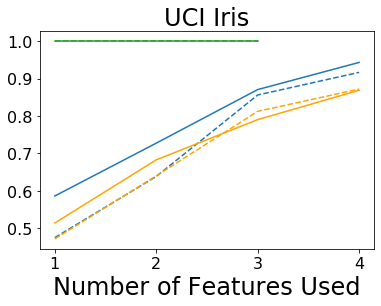
\includegraphics[width=0.24\textwidth]{../openreview/images/tffigures/iris-tradeoff.png}
    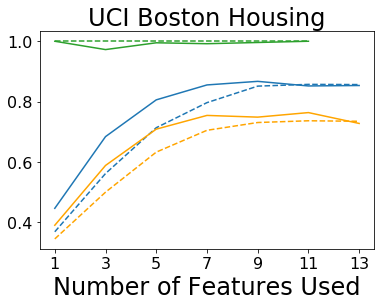
\includegraphics[width=0.24\textwidth]{../openreview/images/tffigures/housing-tradeoff.png}
    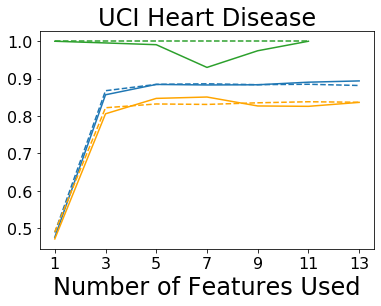
\includegraphics[width=0.24\textwidth]{../openreview/images/tffigures/heart-tradeoff.png}
    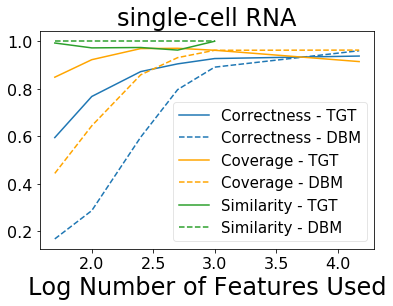
\includegraphics[width=0.24\textwidth]{../openreview/images/tffigures/bipolar-tradeoff.png}
    \caption{Comparison of the metrics(Correctness, Coverage, and Similarity) across different datasets for reproduction experiments.}
    \label{fig:reproduced_tgt_metrics}
\end{figure}
\subsection{Explaining Causal Structure in the Synthetic Data}
We verify the claim that TGT identifies the causal structure in the data (claim 3). The synthetic dataset is generated same as the original paper, i.e. $x_1, x_2 \sim \mathcal{N}(0,0.2) + \rm\ Bern \rm(0.5)$, $x_2 \sim \mathcal{N}(0,0.05), x_4 \sim x_1 + \mathcal{N}(0, 0.05)$. Note that this dataset has four different clusters, caused by the first two dimensions $x_1$ and $x_2$, $x_3$ is noise, and $x_4$ is correlated with $x_1$ and $x_2$. The authors claim that for this synthetic data, TGT is able to find that $x_4$ is not the cause for any group. However, the said claim cannot be re-verified. Interestingly, the re-run of their code doesn't provide the justification either to the degree as mentioned in the paper. We observe that both TGT and DBM are able to identify $x_3$ is not causing any groups. Thus, in this scenario, both TGT and DBM are comparable. Refer table \ref{tab:synth} for the explanations obtained. We, hereby note, that the explanations vary across multiple runs and we use the experimental setup same as the original authors. However, the values across the third dimension are consistently approximately 0.

\subsubsection{Feature modifications}
For each of the UCI datasets, the original authors add a `corrupted' version where an extra cluster is added with artificial feature modification. With the exception of the modified features, the corrupted class is a copy of a chosen target class. They train TGT explanations using both the original scVIS model for the respective dataset and a model retrained on the corrupted dataset. We reproduce these experiments to see if TGT correctly attributes the difference between the target and corrupted class to the right features. 
Refer to Appendix \ref{app:t2c} for the illustrated figures and description. Overall, we observe that TGT is unable to identify the modifications to as good a precision as reported in the original paper. TGT is able to identify the modification for the UCI Iris dataset. For UCI Heart Disease Dataset (figure \ref{fig:t2c-Heart}), it does not identify the features modified and on the UCI Boston Housing Dataset (figure \ref{fig:t2c-Housing}), it identifies noisy modifications. However, with the retrained scVIS model and new representations, TGT is consistent in identifying the modifications across all the datasets. 

% For the UCI Heart Disease dataset, features $6$ and $8$ are modified but TGT identifies those differences to be in features $2, 5$ and $10$. This does not support claim 4. When training TGT on the scVIS model which was trained on the corrupted data, it is able to identify the correct features.

% For the UCI Boston Housing dataset, features $1$ and $9$ are modified. TGT clearly identifies feature $1$ and also identifies feature $9$ but not by the right significance. This does support claim 4. On the retrained scVIS model, the correct features are identified

% For the UCI Iris dataset, feature $1$ was modified, which is correctly identified by TGT on both the original and retrained scVIS model. This supports claim 4.

\subsection{Results beyond original paper}

\subsubsection{PyTorch replication}
We also replicate the TGT algorithm in PyTorch. Our Pytorch implementation includes the entire method along with the scVIS clustering method. In our implementation, we use the Scikit learn \footnote{https://scikit-learn.org/stable/index.html} kmeans module for our cluster selection as opposed to the manual clustering in the Tensorflow implementation. However, our number of clusters argument to the kmeans algorithm was informed by the learned low-dimensional representations for each dataset. Due to differences in the clustering model and cluster selection, we cannot directly compare the coverage and correctness metrics between our Pytorch replication and the TensorFlow reproduction. We additionally experiment with our scaling extension to the TGT algorithm. In the scaling extension of the TGT algorithm, along with the $\delta$ ($\delta$) parameters, each cluster now has a $\gamma$ ($\gamma$) parameters. The transformation from cluster $0$ to $i$ is now given by:
$t_{0 \to i} = e^{\gamma_i} \odot x + \delta_i$
The gammas($\gamma_s$) are truncated just like the deltas and their $L1$ norm is added to the regularization term. Note that these transformations are strictly more expressive. If $\gamma$ is the zero vector, these transformations reduce to regular TGT. 
\subsubsection{UCI Heart Disease and UCI Boston Housing Dataset}
In figure \ref{fig:pt_heart_housing} we see the results of our replication on the UCI Boston Housing and UCI Heart Disease dataset. For the UCI Boston Housing data, the TGT method seems to slightly outperform DBM both with and without scaling. This supports claim 1. The deltas($\delta_s$) and gammas($\gamma_s$) show high similarity, supporting claim 2. For the UCI Heart Disease dataset, we do not see a difference in performance without scaling while TGT with scaling performs slightly worse.
\begin{figure}[H]
    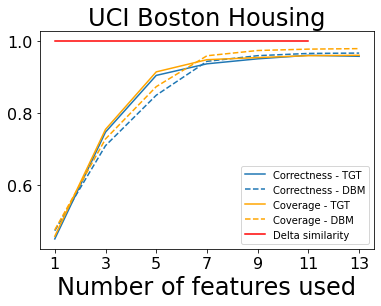
\includegraphics[width=0.24\textwidth]{../openreview/images/ptfigures/housing-tradeoff.png}
    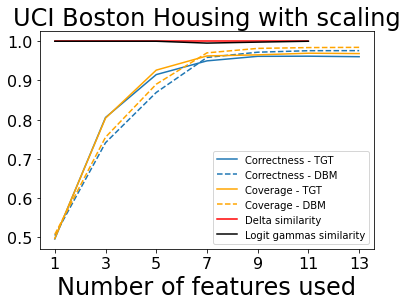
\includegraphics[width=0.244\textwidth]{../openreview/images/ptfigures/housing-scaling-tradeoff.png}
    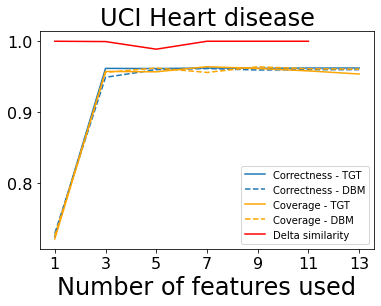
\includegraphics[width=0.24\textwidth]{../openreview/images/ptfigures/heart-tradeoff.png}
    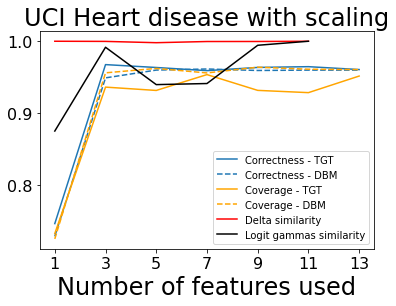
\includegraphics[width=0.24\textwidth]{../openreview/images/ptfigures/heartscaling-tradeoff.png}
    \caption{Results for the PyTorch replication for UCI Boston Housing and UCI Heart Disease dataset.}
    \label{fig:pt_heart_housing}
\end{figure}

\subsubsection{Breast Cancer Wisconsin (Diagnostic) and Pima Indians Diabetes Database}
In figure \ref{fig:pt_diabetes_breast} we see the results for the Pima Indians Diabetes and Breast Cancer Wisconsin (Diagnostic) dataset. For the diabetes dataset, TGT with and without scaling outperforms DBM when more than one feature is used. This supports claim 1. Since the delta ($\delta$) similarity is close to $1$, claim 2 is also supported. For the Breast Cancer dataset, we see similar performance for DBM and TGT and slightly worse performance with scaling. The deltas ($\delta_s$) still have high similarity, supporting claim 2. 

\begin{figure}[H]
    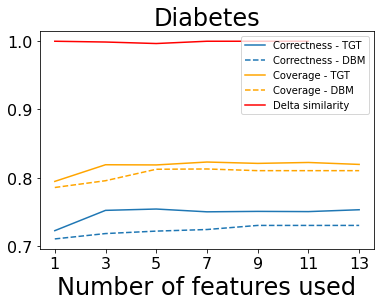
\includegraphics[width=0.25\textwidth]{../openreview/images/ptfigures/diabetes-tradeoff.png}
    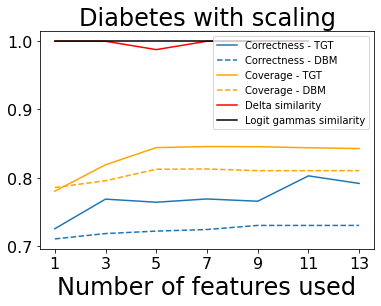
\includegraphics[width=0.24\textwidth]{../openreview/images/ptfigures/diabetes_scaling-tradeoff.png}=
    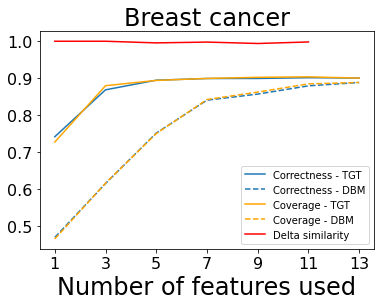
\includegraphics[width=0.24\textwidth]{../openreview/images/ptfigures/breast-tradeoff.png}
    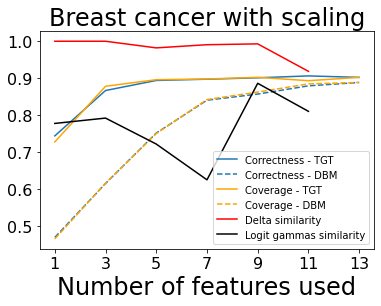
\includegraphics[width=0.24\textwidth]{../openreview/images/ptfigures/breastscaling-tradeoff.png}
    \caption{Results of the PyTorch replication on PIMA Indians Diabetes and Breast Cancer Wisconsin (Diagnostic) Dataset.}
    \label{fig:pt_diabetes_breast}
\end{figure}

\subsubsection{Scaling extension}
% The original authors use translations as their explanation functions. We wonder if these transformation are expressive enough. We replicate our experiment on the housing, heart disease, diabetes and breast cancer datasets. Besides the $\delta$ ($\delta$) parameters, each cluster now has a $\gamma$ ($\gamma$) parameters. The transformation from cluster $0$ to $i$ is now given by:
% $t_{0 \to i} = e^{\gamma_i} \odot x + \delta_i$
% The gammas are truncated just like the deltas and their $L1$ norm is added to the regularization term. Note that these transformations are strictly more expressive. If $\gamma$ is the zero vector, these transformations reduce to regular TGT. 

In figure \ref{fig:pt_heart_housing}, we can see the difference in performance on two dataset included in the original experiments. Scaling does not seem to improve performance on the UCI Boston Housing dataset and slightly decreases performance on the UCI Heart Disease dataset. The similarity of the gammas ($\gamma_s$) is mostly above $0.9$. 

In figure \ref{fig:pt_diabetes_breast},  we see the same metrics for the Breast Cancer and Pima Indians Diabetes Dataset. For the Diabetes dataset, the performance improves slightly and the gammas($\gamma_s$) show high similarity. For the Breast Cancer dataset, the performance is about the same but the gammas($\gamma_s$) show relatively low similarity. 

Altogether, these results suggest that the addition of scaling does not significantly improve the accuracy and correctness while making the transformations more complex. Based on our experiments, we do not recommend the addition of scaling in the explanation functions, and conclude that the original TGT is expressive enough. 

\subsubsection{Experiment with Modified Synthetic Data}
In order to study the efficacy of the proposed scaling function, we perform experiments on the synthetic dataset. We modify one of the groups of points $G$ by performing the operation $ax_{i}^{k} + b$, where $i$ corresponds to the group number and $k$ denotes the feature dimension which we modify. We define $a \sim \mathcal{U}(1.0, 2.0)$  and $b \sim \mathcal{U}(-0.5, 1.0)$. We add modified group $G'$ into the original data $D$ to get the new data $D^{'}$. We follow the experiment setup from the original paper as: a) $r(G^{'})$ should form a different group of its own. b) $G^{'}$ should be within the distribution of the original $D$. In this study, we want to investigate whether the TGT with scaling is able to recover the modifications, and if in doing so it affects the explanations between other groups. The sampling procedure gave a=2.0, b=0.60 and we keep k=0. We observe that the explanations with scaling are able to recover the modification to an approximate degree(scaling factor $e^{\gamma} \approx 2.38$, actual a=2.0), and give better correctness as compared to the regular TGT (refer figure \ref{tab:synth_modified_results}). Interestingly, the translations explanations of the scaling extension are approximately equal to the deltas of the regular TGT. The exact results can be found in Table \ref{tab:synth_modified_results}. Figures \res \ref{fig:synth_modified} and \ref{fig:synth_modified_change} in the appendix show the data spread and resulting translations. 

\begin{table}[]
\scriptsize
\begin{tabular}{|l|l|l|l|l|l|l|l|l|l|l|l|l|}
\hline
 & \multicolumn{2}{c|}{\textbf{0 to 1}} & \multicolumn{2}{c|}{\textbf{1 to 0}} & \multirow{2}{*}{$\delta_1$} & \multirow{2}{*}{$\delta_2$} & \multirow{2}{*}{$\delta_3$} & \multirow{2}{*}{$\delta_4$} & \multirow{2}{*}{$\gamma_1$} & \multirow{2}{*}{$\gamma_2$} & \multirow{2}{*}{$\gamma_3$} & \multirow{2}{*}{$\gamma_4$} \\ \cline{1-5}
 & \multicolumn{1}{c|}{\textit{Cr}} & \multicolumn{1}{c|}{\textit{Cv}} & \multicolumn{1}{c|}{\textit{Cr}} & \multicolumn{1}{c|}{\textit{Cv}} &  &  &  &  &  &  &  &  \\ \hline
\textbf{TGT} & 1 & 0.529 & 0.333 & 1.000 & 2.581 & 0.014 & 0.001 & 0.842 & - & - & - & - \\ \hline
\textbf{Scaling} & 1 & 0.529 & 0.520 & 1.000 & 2.608 & 0.023 & -0.001 & 0.927 & 0.879 & 0.009 & 0.002 & 0.007 \\ \hline
\end{tabular}

\caption{The deltas($\delta_s$) and gammas($\gamma_s$) for the mapping from group 0 to group 1 on the modified synthetic dataset for regular TGT and TGT with scaling. \textit{Cr} and \textit{Cv} indicate correctness and coverage, respectively.}
\label{tab:synth_modified_results}
\end{table}


\subsubsection{Experiments with Probing Classifier}
To further investigate the efficacy of TGT explanations, we use a probing-classifier \cite{belinkov-etal-2020-interpretability} as a proxy to study the qualitative differences of the features selected by TGT and DBM. For each cluster, we train a binary classifier with features ranked highest by TGT and DBM at different sparsity levels K. We compute the overall accuracy at each sparsity level using the ensemble of these binary classifiers.
\begin{figure}
\centering
    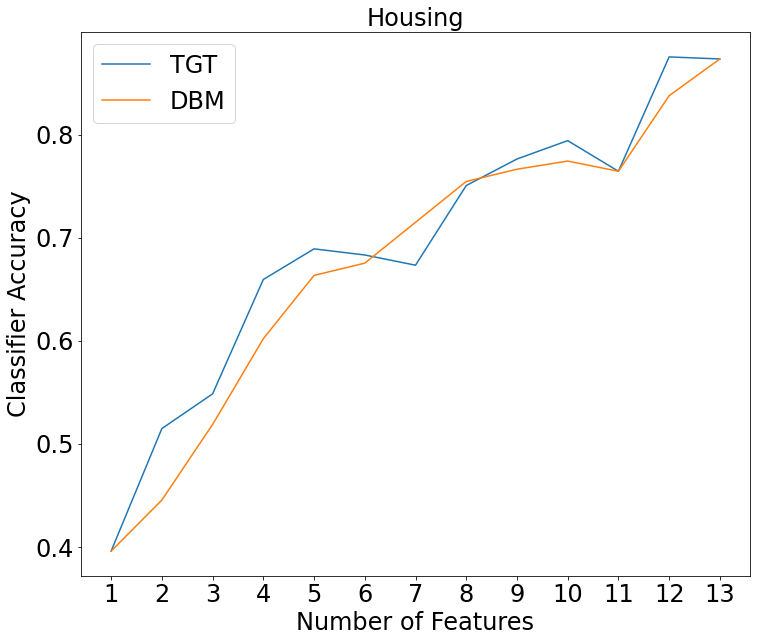
\includegraphics[width=0.3\textwidth, height=3.5cm]{../openreview/images/tffigures/housing-classification-2.png}
    % \hfill
    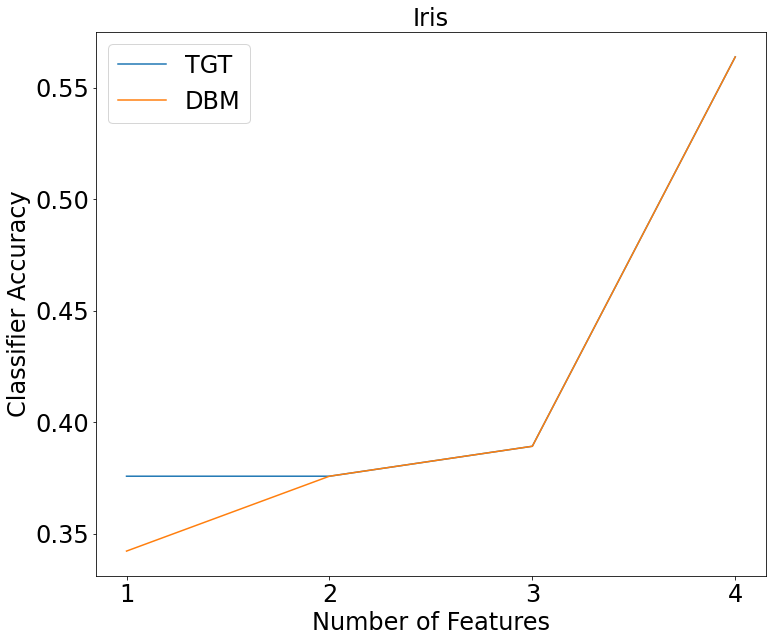
\includegraphics[width=0.3\textwidth, height=3.5cm]{../openreview/images/tffigures/iris-classification-2.png}
    \caption{Classification accuracy of probing classifier at different sparsity levels for Housing (left) and Iris (right) dataset.}
    \label{fig:classification}
\end{figure}
As can be seen in Figure \ref{fig:classification}, the results demonstrate that for sparser explanations, TGT selects features that lead to higher accuracy of the ensemble classifier than those selected by DBM. This further validates the paper’s claim that TGT leads to better sparse explanations as compared to DBM.
Furthermore, we also use the probing classifier to understand the differences between the groups. For each pair of group, we train a Binary Linear Classifier to predict the group of a test point. We, then, investigate the feature importances of the classifier towards decision making. We ascertain that the features classifier give more importance to while decision making are the defining property of the class. Interestingly, we find that the more important features according to the classifier correspond to the explanations provided by the TGT algorithm. Refer to figure \ref{fig:diabetes_1}. This provides further evidence that TGT is able to find real distinctive signals as explanations.



\section{Discussion}
Based on the reproduction of the original experiments, claims 1 and 2 seem to hold, the experiments for claim 4 do not all support it, but the claim does seem to hold. Claim 1 and 2 seem to hold in particular for sparse explanations. The evidence for claim 3 is inconclusive. The coverage and correctness in our reproduction were not always the same as in the original paper. It is difficult to compare these metrics for different clustering outcomes, as they depend on the $\epsilon$ parameter which depends on the clustering.

A major difficulty in reproduction is the cluster selection. When retraining the scVIS model, the latent space representation structure changes. The authors provide no method as to determine the different clusters other than visual inspection. Cluster selection could be an explanation for the differences in results between the original experiments and our reproduction. To verify the results with more confidence, a robust method for cluster selection might be required. 

% \subsection{What was difficult}
% The first difficulty that we encountered was the finding of the right environment. Their code depended on deprecated functionality and could thus not be used with the latest software versions.

% Another difficulty was the selection of clusters. When retraining the scVIS, we get a different latent space representation. The clusters have to be manually selected. This also means there does not have a be a correspondence between the ordering of clusters using the original latent space representation and clusters in the retrained one. Because of this, we cannot compare the metrics between our reproduction and the original experiments.

% \subsection{Communication with original authors}
% We asked the original authors for clarification on how to choose the $\epsilon$ hyper-parameter. However, it became apparent that we had misread, and the procedure is indeed adequately reported in the paper.

%\bibliographystyle{plain}
%\bibliography{bibliography.bib}
% \newpage
